\documentclass[conference]{IEEEtran}
\IEEEoverridecommandlockouts
% The preceding line is only needed to identify funding in the first footnote. If that is unneeded, please comment it out.
\usepackage{cite}
\usepackage{amsmath,amssymb,amsfonts}
\usepackage{algorithmic}
\usepackage{graphicx}
\usepackage{textcomp}
\usepackage{xcolor}
\usepackage[brazilian]{babel}
\usepackage[utf8]{inputenc}
\usepackage[T1]{fontenc}
\usepackage{listings}
\usepackage{color}
\usepackage{float}
\usepackage{multirow}
\usepackage{hyperref}

\definecolor{dkgreen}{rgb}{0,0.6,0}
\definecolor{gray}{rgb}{0.5,0.5,0.5}
\definecolor{mauve}{rgb}{0.58,0,0.82}

\lstset{frame=tb,
  language=Java,
  aboveskip=3mm,
  belowskip=3mm,
  showstringspaces=false,
  columns=flexible,
  basicstyle={\small\ttfamily},
  numbers=none,
  numberstyle=\tiny\color{gray},
  keywordstyle=\color{blue},
  commentstyle=\color{dkgreen},
  stringstyle=\color{mauve},
  breaklines=true,
  breakatwhitespace=true,
  tabsize=3
}
\lstset{language=Python}
\def\BibTeX{{\rm B\kern-.05em{\sc i\kern-.025em b}\kern-.08em
    T\kern-.1667em\lower.7ex\hbox{E}\kern-.125emX}}
\begin{document}

\title{Relatório do Laboratório 8: \\ Imitation Learning com Keras\\
}

\author{\IEEEauthorblockN{Isabelle Ferreira de Oliveira}
\IEEEauthorblockA{\textit{CT-213 - Engenharia da Computação 2020} \\
\textit{Instituto Tecnológico de Aeronáutica (ITA)}\\
São José dos Campos, Brasil \\
isabelle.ferreira3000@gmail.com}
}

\maketitle

\begin{abstract}
Esse relatório documenta a cópia de um movimento de caminhada de um robô humanoide usando a técnica chamada \textit{imitation learning}. Para isso, foi utilizado o \textit{framework} de \textit{Deep Learning} Keras, que facilita o uso do \textit{framework} Tensorflow.
\end{abstract}

\begin{IEEEkeywords}
\textit{Imitation learning}, \textit{deep learning}, Keras, Tensorflow
\end{IEEEkeywords}

\section{Introdução}
\textit{Deep learning} é um tipo de aprendizado de máquina que treina para aprender através do reconhecimento de padrões em várias camadas de processamento. Entre as tarefas possíveis realizáveis estão o reconhecimento de fala, identificação de imagem e previsões, entre outras tarefas realizadas por seres humanos. 

Esse tipo de estratégia possibilita, também, aprender por imitação. Assim, o comportamento desejado (uma política de controle, por exemplo) é copiado usando aprendizado supervisionado.

O \textit{framework} Keras facilita o uso do \textit{framework} Tensorflow para problemas de \textit{Deep learning}, transformando a implementação, treino e resultado da rede neural em chamadas de API. Os pseudo-códigos dessas chamadas podem ser vistos a seguir. Em seguida, será apresentado como isso foi implementado no contexto do laboratório.

\begin{lstlisting}
# Forward Propagation
def forward_propagation(input):
	z[1] = weights[1]input + biases[1]
	a[1] = g[1](z[1])
	z[2] = weights[2]a[1] + biases[2]
	a[2] = g[2](z[2])
	return z, a
\end{lstlisting}

\begin{lstlisting}
# Gradients' Computation
def compute_gradient_back_propagation(inputs, expected_outputs):
	for i in range(len(inputs)):
		input = inputs[i]
		expected_output = expected_outputs[i]
		
		z, a = forward_propagation(input)

		dz[2] = a[2] - expected_output
		weights_gradient[2] += dz[2] a[1].T
		biases_gradient[2] += dz[2]

		dz[1] = weights[2].T dz[2] * derivate(g[1](z[1]))
		weights_gradient[1] += dz[1] input.T
		biases_gradient[1] += dz[1]

	return weights_gradient, biases_gradient
\end{lstlisting}

\begin{lstlisting}
# Back Propagation
def back_propagation(inputs, expected_outputs):
	weights_gradient, biases_gradient = compute_gradient_back_propagation(inputs, expected_outputs)

	weights[1] -= alpha * weights_gradient[1]
	biases[1] -= alpha * biases_gradient[1]
	weights[2] -= alpha * weights_gradient[2]
	biases[2] -= alpha * biases_gradient[2]
\end{lstlisting}

No pseudocódigo acima, \textit{J} é a função para medir a qualidade das soluções candidatas; \textit{m0} e \textit{C0} são a média e a matriz de covariância iniciais da população que será gerada, respectivamente; \textit{m} e \textit{C} são, de forma análoga, a média e a matriz de covariância atuais da população que será gerada, respectivamente; e \textit{mu} é o tamanho da população considerada como "melhores soluções até então".

\section{Implementação do algoritmo}
Para a implementação da rede neural, era necessário preencher a função \textit{forward\underline{\space}propagation()}, \textit{compute\underline{\space}gradient\underline{\space}back\underline{\space}propagation()} e \textit{back\underline{\space}propagation()} da classe \textit{NeuralNetwork}. Essas funções a se completar estavam no código base fornecido \cite{roteiro}.  

Recebendo os valores de \textit{input}, a função \textit{forward\underline{\space}propagation()} foi implementada conforme apresentado no pseudo-código da Introdução, com o detalhe que a função de ativação $g$ de todos os neurônios utilizada foi a \textit{sigmoid}. Além disso, tanto a função \textit{sigmoid} quanto sua derivada já eram fornecidos pelo código base. 

Já na implementação de \textit{back\underline{\space}propagation()}, também foi implementado conforme o sugerido no pseudo-código da Introdução, ou seja, atualizando os valores de pesos e \textit{biases} subtraindo de seu valor um fator de aprendizado \textit{alpha} vezes os gradientes de pesos e \textit{biases}, respectivamente. Esses valores de gradientes são aqueles calculados em \textit{compute\underline{\space}gradient\underline{\space}back\underline{\space}propagation()}, supondo que essa função já foi corretamente implementado. Foi utilizado para \textit{alpha} o mesmo que o sugerido pelo código base. 

Finalmente, para implementar a função \textit{compute\underline{\space}gradient\underline{\space}back\underline{\space}propagation()}, também foi feito de forma bastante semelhante ao apresentado na Introdução, com o detalhe de usar \textit{numpy.multiply} para multiplicar termo a termo os vetores referentes aos pesos e a derivada da função de ativação.

Para testar o funcionamento dessas implementações, foi inicialmente alterado o valor da variável \textit{classification\underline{\space}function} (entre "sum\underline{\space}gt\underline{\space}zero" no arquivo \textit{test\underline{\space}neural\underline{\space}network.py} do código base, gerando imagens dos resultados da classificação de cada \textit{dataset} para cada uma dessas funções (função "soma $>$ 0" e função "xor") usando rede neural.

Já tendo ciência da correta implementação dos algoritmos de aprendizado, foi feito por fim um teste da segmentação de cores, executando o código do arquivo \textit{test\underline{\space}color\underline{\space}segmentation.py}, conforme indicado no roteiro \cite{roteiro}. Os gráficos de resultados tanto dessa segmentação de cores, quanto das funções anteriores, foram apresentados nas Figuras \ref{sum_gt_zero/cost_function_convergence} a \ref{color_segmentation/segmented_image}.

\section{Resultados e Conclusões}

\subsection{Teste das Funções soma > 0 e xor}

O aprendizado com a rede neural foi executado para as duas funções já citadas na seção anterior. Os resultados dessas execuções foram satisfatórios e saíram conforme o esperado, comprovando o correto funcionamento da implementação e a validade da utilização de rede neural com aprendizado supervisionado no aprendizado dessas funções. Esses resultados foram apresentados nas Figuras de \ref{sum_gt_zero/cost_function_convergence} a \ref{xor/neural_net_classification}.

Vale reparar que, nas Figuras \ref{sum_gt_zero/cost_function_convergence} e \ref{xor/cost_function_convergence}, os custos não são sempre decrescentes com o passar das épocas. Isso, entretanto, não configura erro, uma vez que os ruídos nos \textit{dataset} acabam interferindo durante o aprendizado. O resultado continua correto uma vez que a tendência geral é a diminuição desse custo, até a convergência. O mesmo vale, inclusive, para o gráfico da Figura \ref{color_segmentation/cost_function_convergence_segmentation}, que será melhor discutido na subseção seguinte.

A comparação entre as Figuras \ref{sum_gt_zero/dataset} e \ref{sum_gt_zero/neural_net_classification} e entre as Figuras \ref{xor/dataset} e \ref{xor/neural_net_classification} demonstra que a classificação do \textit{dataset} aconteceu de maneira satisfatória.

\begin{figure}[htbp]
\centering
\centerline{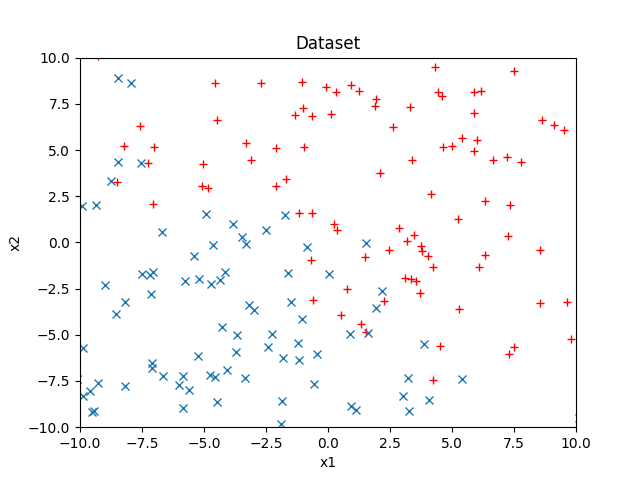
\includegraphics[scale=0.5]{imagens/sum_gt_zero/lambda_zero/dataset_sgz.png}}
\caption{Exemplo de neurônio. Essa imagem de exemplo foi apresentada no roteiro \cite{roteiro}}.
\label{sum_gt_zero/lambda_zero/dataset_sgz}
\end{figure}

\begin{figure}[htbp]
\centering
\centerline{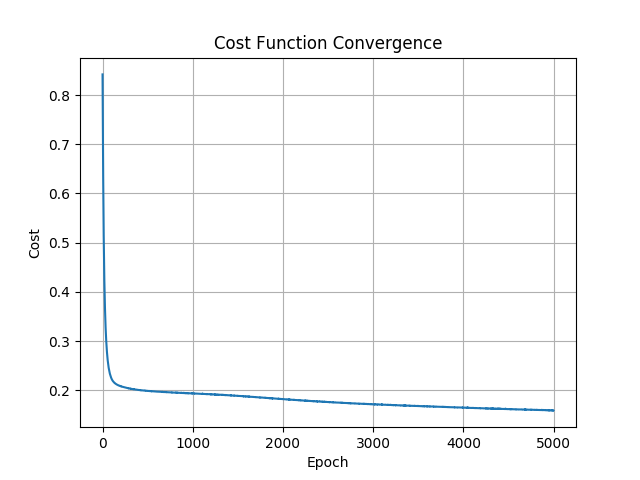
\includegraphics[scale=0.5]{imagens/sum_gt_zero/lambda_zero/convergence_sgz.png}}
\caption{Exemplo de rede neural, com duas camadas (1 camada de entrada, 1 camada escondida e 1 camada de saída), como a trabalhada nesse laboratório. Essa imagem de exemplo foi apresentada no site \cite{neural-net-np}}.
\label{sum_gt_zero/lambda_zero/convergence_sgz}
\end{figure}

\begin{figure}[htbp]
\centering
\centerline{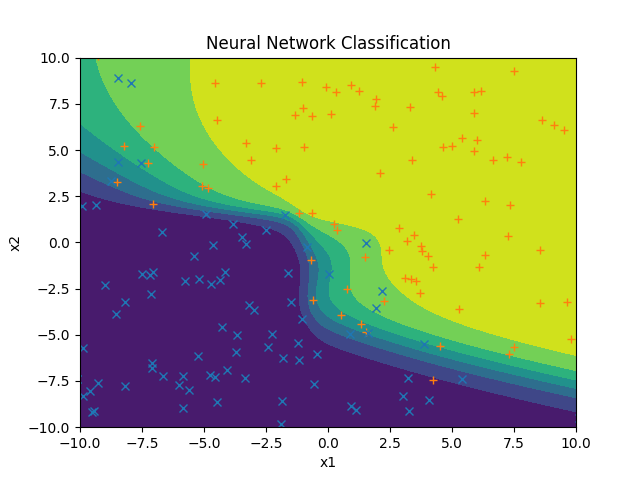
\includegraphics[scale=0.5]{imagens/sum_gt_zero/lambda_zero/nn_classification_sgz.png}}
\caption{Convergência da função de custo para a função \textit{soma > 0}.}
\label{sum_gt_zero/lambda_zero/nn_classification_sgz}
\end{figure}

\begin{figure}[htbp]
\centering
\centerline{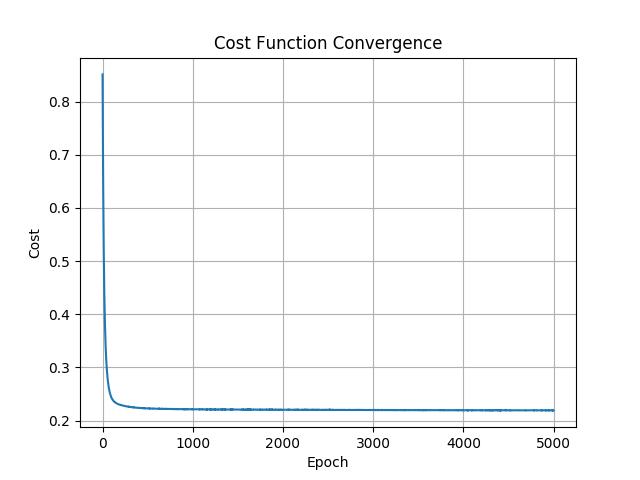
\includegraphics[scale=0.5]{imagens/sum_gt_zero/convergence_sgz.png}}
\caption{\textit{Dataset} utilizado para o aprendizado da função \textit{xor}.}
\label{sum_gt_zero/convergence_sgz}
\end{figure}

\begin{figure}[htbp]
\centering
\centerline{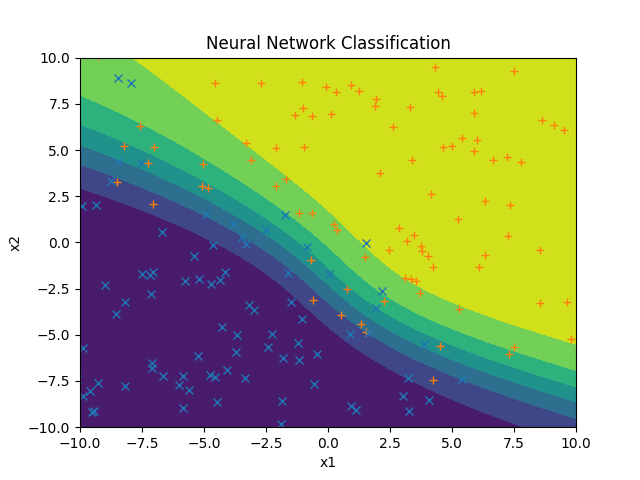
\includegraphics[scale=0.5]{imagens/sum_gt_zero/nn_classification_sgz.png}}
\caption{Convergência da função de custo para a segmentação de cores.}
\label{sum_gt_zero/nn_classification_sgz}
\end{figure}

\begin{figure}[htbp]
\centering
\centerline{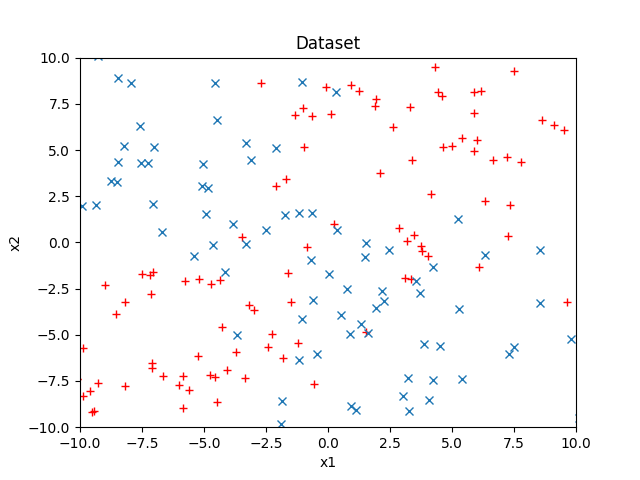
\includegraphics[scale=0.5]{imagens/xor/lambda_zero/dataset_xor.png}}
\caption{Resultado da classificação por rede neural para a função \textit{soma > 0}.}
\label{xor/lambda_zero/dataset_xor}
\end{figure} 

\begin{figure}[htbp]
\centering
\centerline{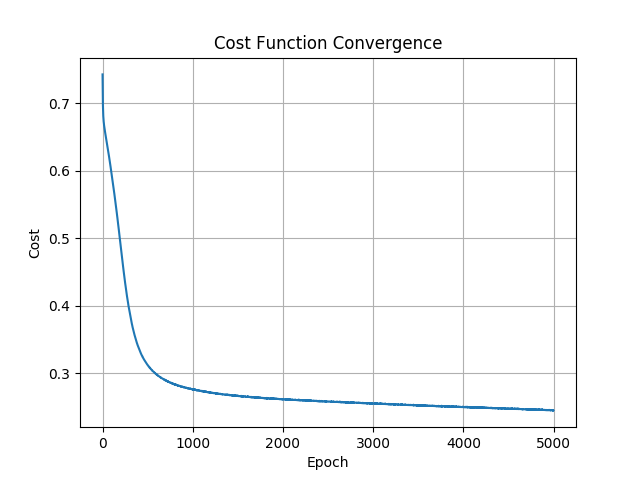
\includegraphics[scale=0.5]{imagens/xor/lambda_zero/convergence_xor.png}}
\caption{\textit{Dataset} utilizado para o aprendizado da função \textit{soma > 0}.}
\label{xor/lambda_zero/convergence_xor}
\end{figure}

\begin{figure}[htbp]
\centering
\centerline{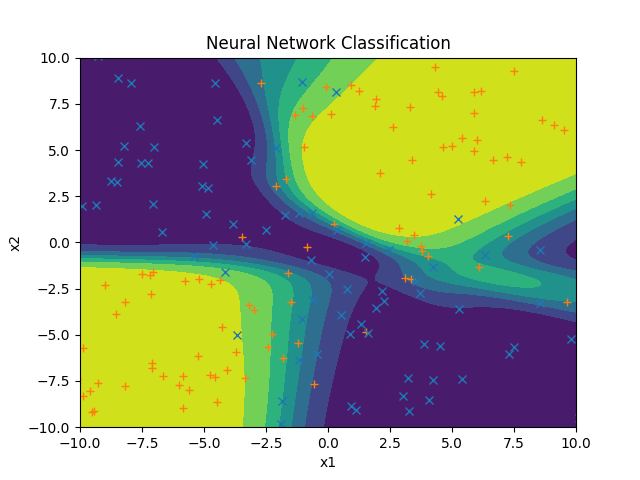
\includegraphics[scale=0.5]{imagens/xor/lambda_zero/nn_classification_xor.png}}
\caption{Convergência da função de custo para a função \textit{xor}.}
\label{xor/lambda_zero/nn_classification_xor}
\end{figure}

\begin{figure}[htbp]
\centering
\centerline{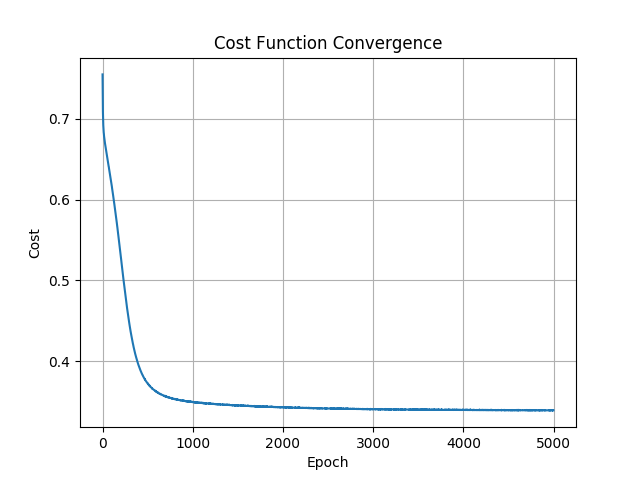
\includegraphics[scale=0.5]{imagens/xor/convergence_xor.png}}
\caption{Imagem original a ter cores segmentadas pela rede neural.}
\label{xor/convergence_xor}
\end{figure}

\begin{figure}[htbp]
\centering
\centerline{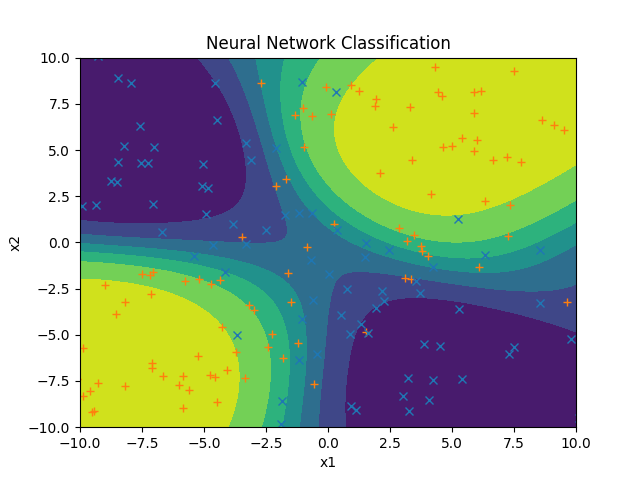
\includegraphics[scale=0.5]{imagens/xor/nn_classification_xor.png}}
\caption{Imagem já com as cores segmentadas pela rede neural.}
\label{xor/nn_classification_xor}
\end{figure}

\subsection{Teste da segmentação de cores}

O custo na Figura \ref{color_segmentation/cost_function_convergence_segmentation} segue a tendência geral de diminuição e convergência com o passar das épocas, apesar de alguns picos já explicados na subseção anterior. Esse resultado é satisfatório e pode ser melhor observado na comparação entre as Figuras \ref{color_segmentation/original_image} e \ref{color_segmentation/segmented_image}, que demonstra que a rede neural realmente conseguiu aprender a classificar as cores verdes e branco com considerável acerto. Vale notar também as cores não identificadas, como a bola laranja, que foi deixada como preta (cor representativa de impossibilidade de identificar).

Tendo em vista o que foi apresentado, pode-se notar, por fim, que esses algoritmos realmente se demonstraram eficazes em encontrar os pesos e \textit{biases} dessa rede neural, além de demonstrar a capacidade de aprendizado de uma rede neural para esses problemas de classificação.

\begin{thebibliography}{00}
\bibitem{roteiro} M. Maximo, ``Roteiro: Laboratório 5 - Estratégias Evolutivas''. Instituto Tecnológico de Aeronáutica, Departamento de Computação. CT-213, 2019.

\bibitem{neural-net-np} Towards Data Science, "Neural Net from scratch". Acessado em https://towardsdatascience.com/neural-net-from-scratch-using-numpy-71a31f6e3675.

\bibitem{sas} SAS, "Redes Neurais: O que são e qual a sua importância?". Acessado em https://www.sas.com/pt\underline{\space}br/insights/analytics/neural-networks.html.

\end{thebibliography}

\end{document}
